\section{The active protocol}
\label{sec:active}

\subsection{Folded states}

Define

\begin{equation}
\ket{L_x}=D_2HD_1\ket{u},
\qquad
\ket{R_x}=HD_3HD_4\ket{u}.
\label{eq:active-folded}
\end{equation}

One photon is prepared in

\begin{equation}
\frac{\ket{0}\ket{L_x}+\ket{1}\ket{R_x}}{\sqrt2},
\end{equation}

where the first register is a path degree of freedom and the second register contains 4096 logical modes. Chronologically, the left path crosses $D_1$, then $H$, then $D_2$, while the right path crosses $D_4$, then $H$, then $D_3$, then a second $H$. Both paths therefore cross exactly two unknown sign banks.

The folded-state overlap is

\begin{equation}
\braket{L_x}{R_x}
=\bra{u}D_1HD_2HD_3HD_4\ket{u}
=\Forr(x).
\label{eq:active-overlap}
\end{equation}

Figure~\ref{fig:active-protocol} gives the physical circuit for one flag. Every unknown sign bank is shown as a two-dimensional phase grid indexed by $(a,b)\in[64]^2$; this coordinate display follows the factorization $4096=64^2$ and does not require the device to use a square spatial array.

\begin{figure*}[t]
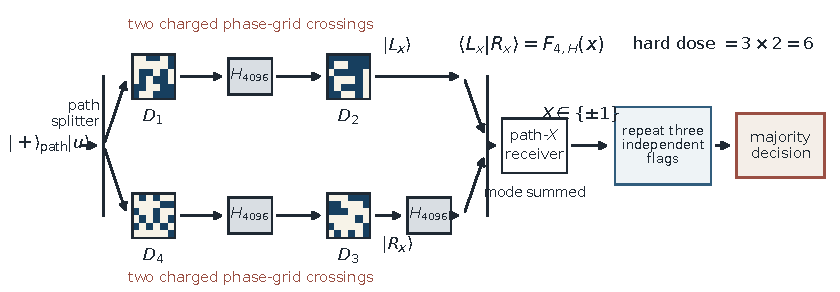
\includegraphics[width=\textwidth]{figures/active_protocol.pdf}
\caption{One active binary flag and the three-flag decision. The left path crosses $D_1$, $H_{4096}$, and $D_2$, while the right path crosses $D_4$, $H_{4096}$, $D_3$, and a second $H_{4096}$. Each path therefore crosses two charged phase grids. Recombination in the path-$X$ basis measures the folded-state overlap while summing over the logical mode coordinate. Three sequential repetitions use the same four sign banks, have total hard dose six, and are decoded by majority. The phase patterns are representative two-dimensional grid icons rather than a restriction on the input law.}
\label{fig:active-protocol}
\end{figure*}

A Pauli-$X$ measurement on the path produces a binary flag $X\in\{\pm1\}$ with

\begin{equation}
\mathbb E[X\mid x]=\Forr(x).
\end{equation}

The mode register need not be resolved at the receiver; the two paths are recombined, the output port is detected, and the mode label is summed over.

\subsection{Error and dose}

At either promise boundary, one flag is correct with probability $5/8$. Three independent flags followed by majority decoding have worst-case error

\begin{equation}
\left(\frac38\right)^3
+3\left(\frac58\right)\left(\frac38\right)^2
=\frac{81}{256}
=0.31640625.
\end{equation}

The exact margin below $1/3$ is

\begin{equation}
\frac13-\frac{81}{256}=\frac{13}{768}.
\end{equation}

For example, the retained detector record $(+1,-1,+1)$ is decoded as the positive promise side. Every one of the three flags remains in the record, so the majority rule uses no favorable-outcome filtering or postselection.

Each flag uses deterministic hard dose two, and the three retained flags use deterministic hard dose six. The protocol has no postselection, and all no-click or erased outcomes must remain in the decision record under a nonideal implementation.

\begin{table}[t]
\caption{Active resource ledger at $N=4096$.}
\label{tab:active-resources}
\begin{ruledtabular}
\begin{tabular}{lc}
Resource & Requirement \\
\colrule
Sign banks & $4$ \\
Sign coordinates & $16{,}384$ \\
Logical mode dimension & $4096$ \\
Path dimension & $2$ \\
Single-photon flags & $3$ \\
Charged traversals per flag & $2$ \\
Total hard dose & $6$ \\
Receiver & path-$X$, mode insensitive \\
Postselection & none \\
\end{tabular}
\end{ruledtabular}
\end{table}

The three flags may use the same optical network sequentially, so the resource statement does not require three copies of the sign banks or public transforms.
